\documentclass[a4paper,12pt,oneside]{report}

% ------------------------------------------------
% LANGUAGE & FONTS
% ------------------------------------------------
\usepackage[british]{babel}
\usepackage[T1]{fontenc}
\usepackage[utf8]{inputenc}
\usepackage{newtxtext,newtxmath} % Times New Roman-like fonts for pdflatex

% ------------------------------------------------
% PAGE GEOMETRY
% ------------------------------------------------
\usepackage[a4paper,
    left=3.5cm,
    right=1.25cm,
    top=2.5cm,
    bottom=1.25cm
]{geometry}

% ------------------------------------------------
% LINE SPACING & INDENTATION
% ------------------------------------------------
\usepackage{setspace}
\doublespacing
\setlength{\parindent}{1.25cm}

% ------------------------------------------------
% CHAPTER, SECTION, SUBSECTION FORMATTING
% ------------------------------------------------
\usepackage{titlesec}
% Chapter Title - 16pt, Bold, Capital, Centered
\titleformat{\chapter}[block]
  {\centering\normalfont\bfseries\fontsize{16}{20}\selectfont}
  {\thechapter.}{1em}{\MakeUppercase}

% Section - 14pt, Bold
\titleformat{\section}
  {\normalfont\bfseries\fontsize{14}{16}\selectfont}{\thesection}{1em}{}

% Subsection - 12pt, Bold
\titleformat{\subsection}
  {\normalfont\bfseries\fontsize{12}{14}\selectfont}{\thesubsection}{1em}{}

% ------------------------------------------------
% CAPTION SETTINGS
% ------------------------------------------------
\usepackage{caption}
\captionsetup[figure]{
    font={it,small},
    labelfont={bf},
    labelsep=period,
    justification=centering,
    name=Figure
}
\captionsetup[table]{
    font={it,small},
    labelfont={bf},
    labelsep=period,
    justification=centering,
    name=Table,
    position=top
}

% ------------------------------------------------
% NUMBERING FORMAT
% ------------------------------------------------
\numberwithin{equation}{chapter}
\numberwithin{figure}{chapter}
\numberwithin{table}{chapter}

% ------------------------------------------------
% OTHER PACKAGES
% ------------------------------------------------
\usepackage{graphicx}
\usepackage{amsmath}
\usepackage{listings}
\usepackage{float}
\usepackage{makeidx}
\usepackage{hyperref}
\usepackage{xcolor}
\usepackage{microtype}

\lstset{
    basicstyle=\ttfamily\footnotesize,
    breaklines=true
}

% ------------------------------------------------
% TITLE PAGE
% ------------------------------------------------
\begin{document}

\begin{titlepage}
\begin{center}
    \Large\textbf{FOUR WEEK TRAINING REPORT}\\[3mm]
    \large{at}\\[3mm]
    \Large\textbf{Academic Advancement of Information Technology, Mohali}\\[6mm]
    \normalsize{SUBMITTED IN PARTIAL FULFILLMENT OF THE REQUIREMENTS FOR THE AWARD OF DEGREE OF}\\[3mm]
    \Large\textbf{BACHELOR OF TECHNOLOGY}\\[3mm]
    \large{in Computer Science and Engineering}\\[9mm]
    
\includegraphics[height=6cm]{gndeclogo.png}\\[6mm]
    \large{JUNE–JULY 2025}\\[9mm]
    \textbf{SUBMITTED BY:}\\
    NAME: Ayush Mehta\\
    UNIVERSITY ROLL NO.: 2302489
\end{center}

\vspace{10mm}
\begin{center}
    \textbf{Department of Computer Science and Engineering}\\
    \textbf{Guru Nanak Dev Engineering College}\\
    \textbf{Ludhiana, 141006}
\end{center}
\end{titlepage}

% ------------------------------------------------
% CERTIFICATE PAGE (TO BE INSERTED FROM COMPANY)
% ------------------------------------------------
\newpage
\begin{center}
    \large\textbf{CERTIFICATE}\\[6mm]
    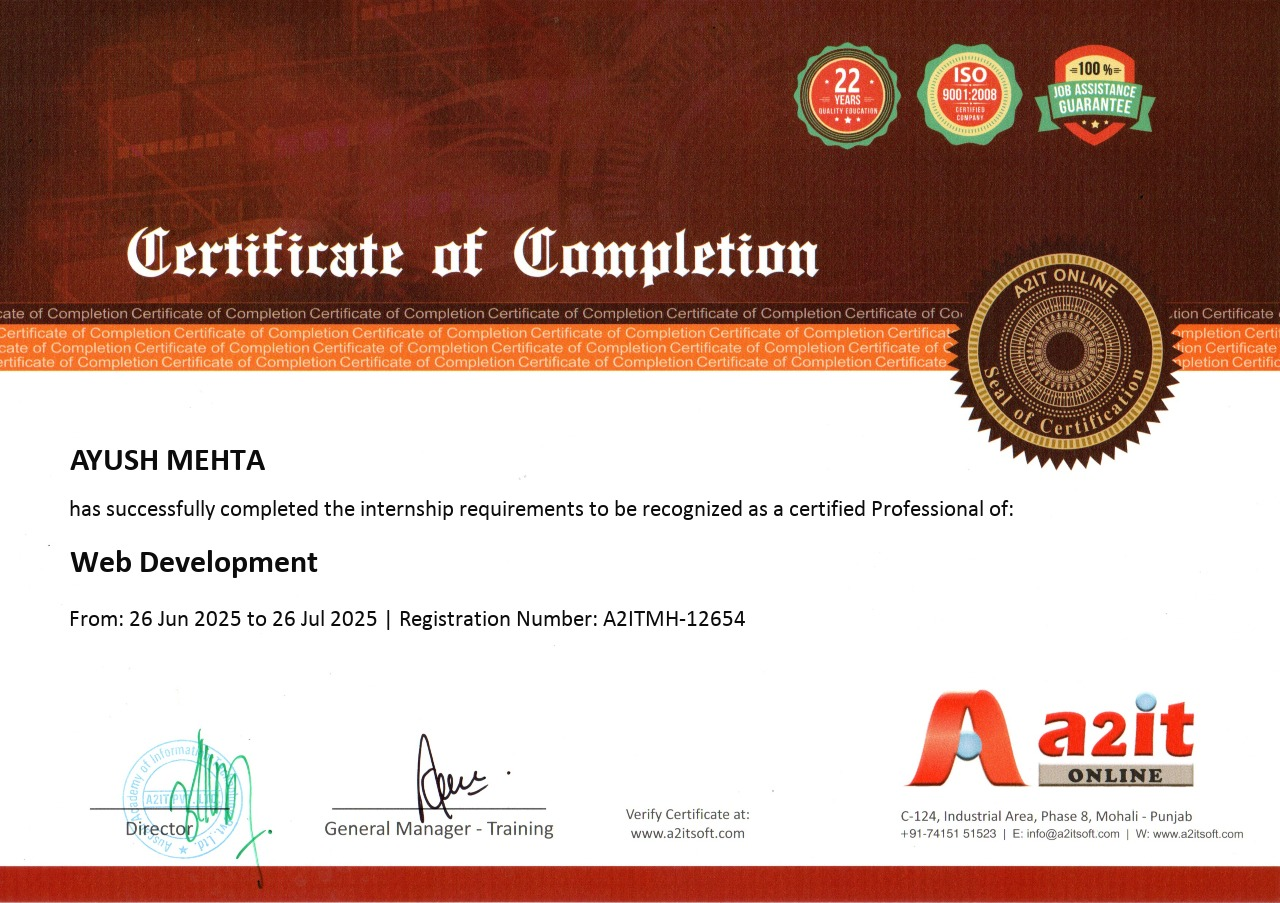
\includegraphics[width=\textwidth, keepaspectratio]{certificate.jpg}
\end{center}

% ------------------------------------------------
% CANDIDATE’S DECLARATION
% ------------------------------------------------
\newpage
\begin{center}
    \large\textbf{CANDIDATE'S DECLARATION}
\end{center}

I, \textbf{Ayush Mehta}, hereby declare that I have undertaken four-week Web Development training from \textbf{Academic Advancement of Information Technology, Mohali} during the period from 26 June 2025 to 26 July 2025 in partial fulfillment of the requirements for the award of the degree of \textbf{B.Tech. (Computer Science and Engineering)} at \textbf{Guru Nanak Dev Engineering College, Ludhiana}. The work presented in this training report is an authentic record of my training.

\vspace{15mm}
\noindent
\textbf{(Ayush Mehta)}\\
Roll No.: 2302489\\[10mm]
The four week industrial training Viva--Voce Examination of \rule{4cm}{0.4pt} has been held on \rule{3cm}{0.4pt} and accepted.

\vspace{45mm}

\noindent
\begin{tabular}{p{0.45\textwidth}p{0.45\textwidth}}
\centering\textbf{Signature of External Examiner} & \centering\textbf{Signature of Internal Examiner} \\
\end{tabular}

% ------------------------------------------------
% ABSTRACT
% ------------------------------------------------
\newpage
\begin{center}
    \large\textbf{ABSTRACT}
\end{center}

This report summarizes the four-week industrial training in Web Development undertaken at \textbf{Academic Advancement of Information Technology (A2IT), Mohali}. The training primarily focused on learning the fundamentals of front-end web technologies, including \textbf{HTML} and \textbf{CSS}, along with an introductory understanding of \textbf{JavaScript}. 

As a beginner to web development, this training provided me with a strong foundation in creating structured, styled, and responsive web pages. The sessions covered essential concepts of website design and layout, enabling me to understand how the various components of a web application interact. 

Towards the end of the training, I developed a small project—a \textbf{Scientific Web Calculator}—which allowed me to apply the knowledge gained during the sessions. Although simple, this project served as a practical exercise to consolidate the learning outcomes. Overall, the training proved to be an invaluable starting point for my journey into web development and helped me build confidence in working with core web technologies.

% ------------------------------------------------
% ACKNOWLEDGEMENT, CONTENTS, ETC.
% ------------------------------------------------

\newpage
\begin{center}
    \large\textbf{ACKNOWLEDGEMENT}
\end{center}

I express my deepest sense of gratitude to \textbf{Dr.~Sehijpal Singh}, Principal, Guru Nanak Dev Engineering College, Ludhiana, for providing the necessary facilities and environment for carrying out the training successfully. I am equally thankful to \textbf{Dr.~Kiran Jyoti}, Head, Department of Computer Science and Engineering, for her valuable support, motivation, and guidance during the course of the training.

I am sincerely thankful to \textbf{Mr.~Jaswant Singh} and \textbf{Ms.~Kuljit Kaur}, Training Coordinators, Department of Computer Science and Engineering, for their constant guidance, encouragement, and for providing valuable instructions regarding the preparation of this report and the training documentation.

I would also like to express my heartfelt thanks to the management and staff of \textbf{Academic Advancement of Information Technology (A2IT), Mohali} for providing me the opportunity to undergo industrial training. I extend my sincere appreciation to \textbf{Ms.~Payal Karn} for her continuous guidance, insightful lectures, and support throughout the training period. I am also thankful to \textbf{Mr.~Rajeev}, Director of Technology, A2IT, for facilitating the overall training program, and to \textbf{Ms.~Harpreet Kaur}, Senior Manager (Human Resources), A2IT, for her assistance in administrative and certification matters.

Lastly, I extend my gratitude to all my faculty members, friends, and family who directly or indirectly helped me during this training and in preparing this report.

\vspace{10mm}
\noindent
\textbf{(Ayush Mehta)}\\
Roll No.: 2302489

\tableofcontents
\listoffigures
\listoftables

% ------------------------------------------------
% CHAPTERS
% ------------------------------------------------
\chapter{INTRODUCTION}
Write your introduction here.

\chapter{TRAINING WORK UNDERTAKEN}
Write about the training tasks, technologies, and projects.

\chapter{RESULTS AND DISCUSSIONS / OBSERVATIONS}
Include screenshots, tables, and analysis.

\chapter{CONCLUSION}
Summarize the work and key learnings. (Should not exceed one page.)

% ------------------------------------------------
% REFERENCES
% ------------------------------------------------
\newpage
\begin{thebibliography}{9}
\addcontentsline{toc}{chapter}{References}
\bibitem{ref1} Author Name, \textit{Book Title}, Publisher, Year.
\bibitem{ref2} Website or article reference.
\end{thebibliography}

% ------------------------------------------------
% APPENDIX
% ------------------------------------------------
\appendix
\chapter*{APPENDIX}
(Include any additional material, code, or data here.)

\end{document}
